\documentclass{article}

\usepackage{graphicx}

\usepackage{hyperref}

\title{Coordinate spaces\\\large{OpenGL and tangent space normal mapping}}
\author{Yotam Gingold\\
George Mason University\\
\emph{ygingold@gmu.edu}}
\date{}

\begin{document}
\maketitle

%% window coordinates <--viewport-- normalized device <--projection-- eye-space <--modelview-- world-space
%% Texture space (uv/st) and tangent space.   Remind about packing normals in a texture.

\section{Positions}
\begin{figure*}
\centering
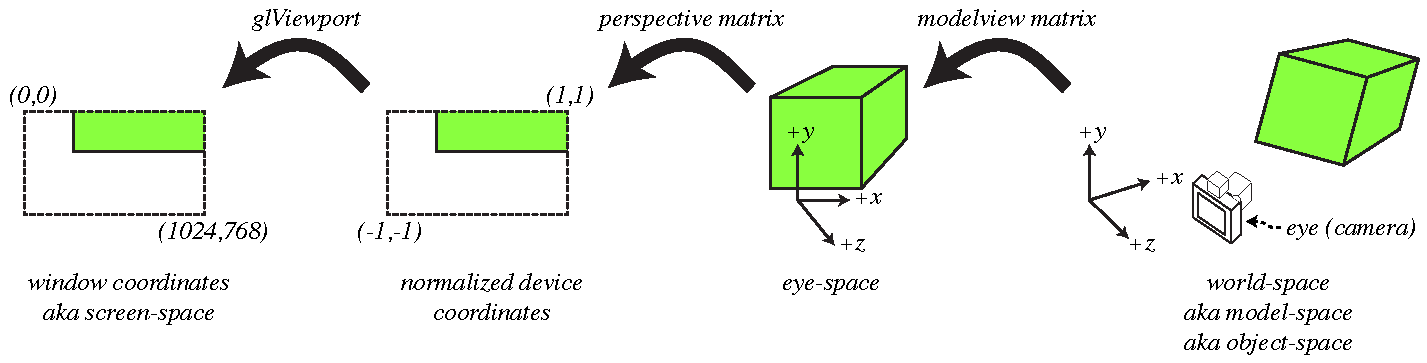
\includegraphics[width=\textwidth]{figures/positions}
\end{figure*}

Let's load an \verb|OBJ| file containing a 3D model.
Every vertex of the 3D model has a position $p$; we usually
label the three coordinate axes of $p$ as $x,y,z$.  Then we can say that
the vector $(1,0,0)$ points in the $+x$ direction (and has unit length),
the vector $(0,1,0)$ points in the $+y$ direction, and
the vector $(0,0,1)$ points in the $+z$ direction.
We usually also call the position whose coordinates are $(0,0,0)$ the \emph{origin}.

Let's pretend that the model we load is a cube centered around the origin ($(0,0,0)$),
and let's pretend that edges of the cube are aligned with the coordinate axes ($x,y,z$).
Where does that put the cube in relation to us?  Is $(0,0,0)$ at the center of the earth?
The center of the sun?  The center of our galaxy?  Which way is $+x$?
Your right?

This is a trick question.  The cube lives in one coordinate space,
we live in a different one, and there is no absolute origin or
absolute $+x, +y,$ or $+z$ directions.
Everything is \emph{relative}; the best we can do is say
where the origin and $+x, +y, +z$ directions of one coordinate space are
relative to another coordinate space's origin and $+x,+y,+z$ directions.
(Actually, we will be talking about where the unit $+x$, unit $+y$, and unit $+z$
coordinate axes of one coordinate space are in terms of another's, because
the two coordinate spaces may have different relative sizes.)

Continuing with our cube example, let's say that relative to where you are
standing---in your ``eye-space'' coordinate frame, where your head is
located at the origin, $+x$ is to the right, $+y$ is up, and $+z$ is behind
you---the cube is centered around $(0, 0, -3)$ and its edges are aligned
with $(\frac{1}{2},\frac{1}{2},0)$, $(-\frac{1}{2}, \frac{1}{2}, 0)$, and
$(0,0,\frac{1}{\sqrt{2}})$.  Then to convert from the cube's coordinate frame
to eye-space, we need to scale the edges of the cube by $\frac{1}{\sqrt{2}}$,
rotate $45$ degrees counterclockwise about the $+z$ axis,
and finally translate by $(0, 0, -3)$.
Translation, rotation, and scaling are all linear transformations,
so we can represent this coordinate transformation as multiplication
by a $4$-by-$4$ matrix.
(The matrix is $4$-by-$4$ and not $3$-by-$3$ because translations
are handled via homogeneous coordinates.  Points are given
a fourth, $w$ component which is always $1$: $x, y, z, 1$.
Vectors have no fixed position and cannot be translated,
so they are given a $w$ component always equal to $0$;
equivalently, the vector can be multiplied by the upper-left
$3$-by-$3$ sub-matrix.)

Eye-space is a convenient coordinate system.  In eye-space, the eye/head/camera
is located at $(0,0,0)$, which is convient for lighting calculations where you
need to know the direction towards the eye.
In eye-space, right is $+x$, up is $+y$, and forward is $-z$.
The coordinate transformation that converts the raw vertices you pass
to OpenGL from their coordinate space (variably called object-space, model-space,
or world-space) into eye-space is called the ``modelview'' matrix.

Before we move on, a note on normal vectors.
Normal vectors are not ``typical'' vectors,
because they are defined as the direction perpendicular to a surface.
If you have a transformation matrix $M$ that converts from one coordinate
space to another (such as your modelview matrix),
then the matrix for transforming normals---it preserves
the perpendicularity of the normal---is ${M^{-1}}^T$.  If you work it out,
you will see that this performs the same rotation as $M$ but performs
the inverse scaling.

The next coordinate space of interest in OpenGL is called \emph{normalized
device coordinates}.  In this coordinate space, the lower-left corner
of the rectangular portion of the screen to which you are drawing
has $(x,y)$ coordinates $(-1, -1)$ and the upper-right corner has
$(x,y)$ coordinates $(1,1)$.
(The center of the rectangle has $(x,y)$ coordinates $(0,0)$.)
Anything outside this rectangle will be clipped and not drawn.
Similarly, the depth component ($z$) runs from $-1$ to $1$, where
something with $z=-1$ is in front of something with $z=1$; anything
with $z$ outside of this range is clipped.
The coordinate transformation that transforms from eye-space to normalized device
coordinates is called the projection matrix.  Often you will specify \emph{near}
and \emph{far} clipping planes; an eye-space point with $z=-near$ is transformed
into a normalized device coordinate point with $z=-1$,
and an eye-space point with $z=-far$ is transformed
into a normalized device coordinate point with $z=1$.

The final coordinate space in the OpenGL rendering pipeline is called window coordinates.
In window coordinates, the lower-left corner of the portion
of the screen to which you are drawing has coordinates $(0,0)$,
and the upper-right corner of the portion of the screen to which you are drawing
has coordinates $(width, height)$, where $width$ and $height$ are in units of
pixels.  In window coordinates, depth ranges from $z=0$ (close) to $z=-1$ (far).
The window coordinate space is sometimes called screen-space.
The parameters to $glViewport()$ define the window coordinates.

\section{Texture coordinates}
\begin{figure*}
\centering
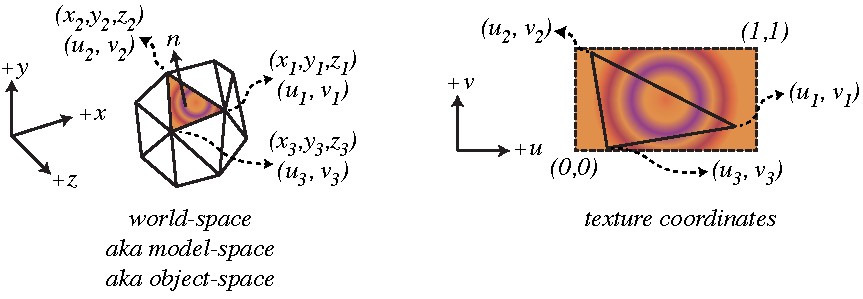
\includegraphics[width=\textwidth]{figures/texcoords}
\end{figure*}

So far we have discussed all of the notable coordinate spaces in OpenGL
that are used to determine the screen-space position coordinates of a (raw)
world-space vertex position.  However, there are another set of coordinates
used in texture mapping called \emph{texture coordinates}.  In addition
to $x,y,z$ world-space coordinates, every vertex also has 2D texture
coordinates, usually denoted $u,v$ or $s,t$, where $(0,0)$ is the lower-left
corner of the 2D texture image and $(1,1)$ is the upper-right corner.
(Since texture coordinates and positions are defined at vertices,
the texture coordinates and positions inside each triangle are
obtained by linearly interpolating the texture coordinates and positions
of the vertices of the triangle.)
Texture coordinates run tangent to (along) the surface, so we can define
\emph{tangent-space} to be the varying coordinate space---defined at any
position on the surface---whose coordinate axes are $+u, +v, +n$, where
$+u$ is called the tangent vector, $+v$ is called the bi-tangent vector,
and $+n$ is the normal to the surface.

In tangent-space bump mapping, a greyscale texture $B$ is interpreted as
the amount the surface is displaced along the normal direction.
However, we don't actually displace the surface in bump mapping; instead, we
compute the normal of the would-be displaced surface and use that for our
lighting computation.  So all we need to know is the normal of the would-be
displaced surface, which is
$( -\frac{\partial{B}}{\partial u}, -\frac{\partial{B}}{\partial v}, 1 )$.

In tangent-space normal mapping, a color texture $N$ stores
tangent-space normal vectors $(u,v,n)$.
(Although it is an implementation detail, note that $r,g,b$ color textures
store the $u,v,n$ normal coordinates by shifting and scaling the $r,g,b$
colors, which lie in the range $[0,1]$, into the range $[-1,1]$, where
the coordinates of normal vectors lie.)

To convert from tangent-space to eye-space, where lighting is conveniently
performed, we need a way to map $u,v,n$ coordinates into eye-space.
In other words, we need to find the unit $+u$ and $+v$ directions
in eye-space.
We have to do this correctly, or else adjacent pixels will have normals
that appear to ``twist'' in weird ways.

One way to find $+u$ and $+v$ in eye-space is to first find them in world-space.
We know what the world-space $x,y,z$
coordinates are for every vertex of a triangle, and what the $u,v$ coordinates
are, too.  The world-space $x,y,z$ coordinates for $+u$ and $+v$ are six unknowns,
but we have enough equations in the form of the world-space vectors and
texture coordinate vectors along the edges of the triangle.
With a little bit of algebra, we can determine per-triangle $+u$ and $+v$ vectors
in world-space.  Then, just as per-vertex normals can be
computed by averaging the normals of the triangles that meet at each vertex,
per-vertex tangent ($+u$) and bi-tangent ($+v$) vectors can be computed.
World-space tangent and bi-tangent vectors can be converted to eye-space
vectors by multiplying with the modelview matrix (not its inverse-transpose;
that's only for perpendicular vectors).

Another way to find the $+u$ and $+v$ in eye-space is via a coordinate
transformation to screen-space.  In the OpenGL fragment shader,
we have available the functions $dFdx()$ and $dFdy()$, which
will tell us how a value changes along the $+x$ or $+y$
window coordinate (screen-space) directions, respectively.
We can use $dFdx()$ and $dFdy()$ on the texture coordinates
and on the eye-space vertex position; then, with a little bit of algebra, we
can determine the per-pixel $+u$ and $+v$ vectors in eye-space.



\section{Tip: the columns of a matrix}
If you are dealing with vectors, such as normals and tangents and bi-tangents,
then you don't need to worry about translation.
In that case, consider the matrix
\[
    M = \left[ \begin{array}{ccc}x_1 & x_2 & x_3 \\ y_1 & y_2 & y_3 \\ z_1 & z_2 & z_3\end{array} \right]
\]
If you multiply $M$ on the right by the vector $( 1, 0, 0 )$ in the form of a column matrix $[ 1, 0, 0 ]^T$, you get $[ x_1, y_1, z_1 ]^T$.
Similarly, if you multiply $M$ on the right by the vector $( 0, 1, 0 )$ or $( 0, 0, 1 )$,
you get $[ x_2, y_2, z_2 ]^T$ or $[ x_3, y_3, z_3 ]^T$, respectively.
So the vector $( 1, 0, 0 )$ in the coordinate space on the right of $M$ becomes
the first column of $M$, $( x_1, y_1, z_1 )$ after transformation, and so on.
It follows then that $M^{-1}$ transforms $( x_1, y_1, z_1 )$ into the vector $( 1, 0, 0 )$.
You can arrange the vectors that convert to a coordinate space $W$ from
a coordinate space $S$ as the columns of a matrix and convert $S$ vectors
into $W$ vectors by left-multiplying the matrix with an $S$ vector,
and $W$ vectors into $S$ vectors
by left-multiplying the inverse matrix by a $W$ vector. That's useful!
And if you don't need to go both directions, you don't need the inverse of the matrix,
which is handy if your coordinate spaces have different numbers of coordinates.

In our case, we want to find a tangent frame. With the above framework in mind, we are looking for the (columns of a) matrix that will convert a vector from tangent-space to object-space. We know how we want this matrix to behave for a single triangle with positions and tangent-space (texture) coordinates.
We want the tangent-space vector $( u_2 - u_1, v_2 - v_1, 0 )$ to map to the 3D edge of the triangle $( x_2 - x_1, y_2 - y_1, z_2 - z_1 )$.
We want the tangent-space vector $( u_3 - u_1, v_3 - v_1, 0 )$ to map to the 3D edge of the triangle $( x_3 - x_1, y_3 - y_1, z_3 - z_1 )$.
Finally, we want the tangent-space vector $( 0, 0, 1 )$ to map to the 3D normal to the triangle $( n_x, n_y, n_z )$. We can set this up as a system of equations:

\[
M \left[ \begin{array}{ccc} u_2 - u_1 & u_3 - u_1 & 0 \\ v_2 - v_1 & v_3 - v_1 & 0 \\ 0 & 0 & 1\end{array} \right]
=
\left[ \begin{array}{ccc} x_2 - x_1 & x_3 - x_1 & n_x \\ y_2 - y_1 & y_3 - y_1 & n_y \\ z_2 - z_1 & z_3 - z_1 & n_z \end{array} \right]
\]

Let
\[
W = \left[ \begin{array}{ccc} u_2 - u_1 & u_3 - u_1 & 0 \\ v_2 - v_1 & v_3 - v_1 & 0 \\ 0 & 0 & 1\end{array} \right]
\]
and
\[
S = \left[ \begin{array}{ccc} x_2 - x_1 & x_3 - x_1 & n_x \\ y_2 - y_1 & y_3 - y_1 & n_y \\ z_2 - z_1 & z_3 - z_1 & n_z \end{array} \right]
\]

Then we can find $M = S W^{-1}$.
The columns of $M$ are the tangent frame of the triangle. The first column is the tangent, the second column is the bi-tangent, and the third column is the normal. That's it!
You can use $M$ to convert any tangent-space vector into object-space.
To have a smoothly varying tangent-frame, average the tangent frame (tangent, bi-tangent, and normal) of all triangles incident to a vertex.
Just like with normals, be sure to normalize the tangent and bi-tangent vectors before adding them and at the end.

(Because we already know the normal, we can actually compute the upper-left $2 \times 2$ portion of $W$ and the left two columns of $S$ and still get the tangent and bi-tangent columns of $M$.)

\end{document}
